\documentclass{article}
\usepackage{ctex}
\usepackage{graphicx}
\usepackage{amsmath}
\usepackage{indentfirst}
\usepackage{titlesec}
\usepackage{setspace}
\usepackage{subfigure}
\usepackage{caption}
\usepackage{float}
\usepackage{booktabs}
\usepackage{geometry}
\usepackage{multirow}
\geometry{left=1.2cm,right=1.2cm,top=2cm,bottom=2cm}
\title{\songti \zihao{2}\bfseries HW5三次样条插值}
\titleformat*{\section}{\songti\zihao{4}\bfseries}
\titleformat*{\subsection}{\songti\zihao{5}\bfseries}
\renewcommand\thesection{\arabic{section}}
\author{王启骅 PB20020580}
\begin{document}
	\maketitle
	\section{实验结果分析}
	利用大M法,并用追赶法求解线性方程组得到的结果带入多项式方程S(x)后解出表达式为图1
		\begin{figure}[!h]
		
		\centering
		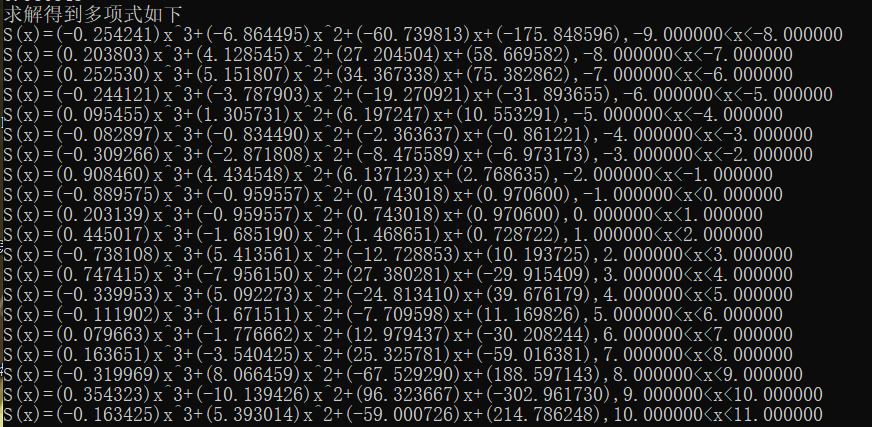
\includegraphics[scale=1]{Sx}
		\captionsetup{font={small},labelfont=bf}
		\caption{\heiti\zihao{-5}S(x)}
		
	\end{figure}
	
	
	改变第10个压铁坐标后求解得到的S(x)表达式为图2
		\begin{figure}[!h]
		
		\centering
		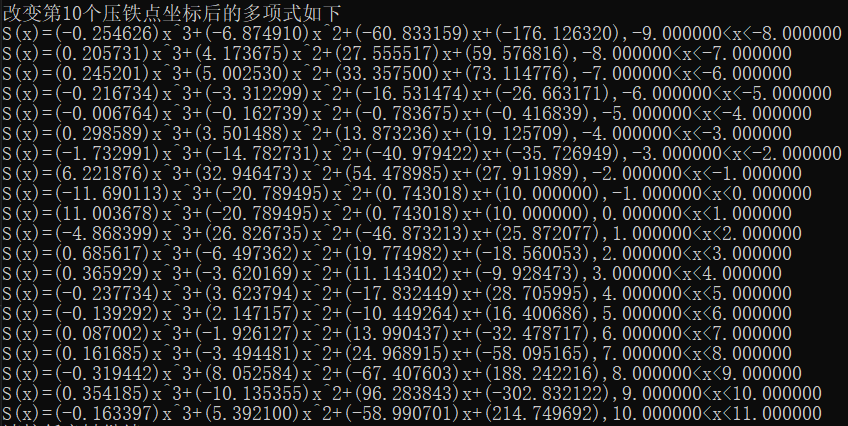
\includegraphics[scale=1]{Sx_1}
		\captionsetup{font={small},labelfont=bf}
		\caption{\heiti\zihao{-5}S(x)}
		
	\end{figure}


将两次结果画图得到图3
	\begin{figure}[!h]
	
	\centering
	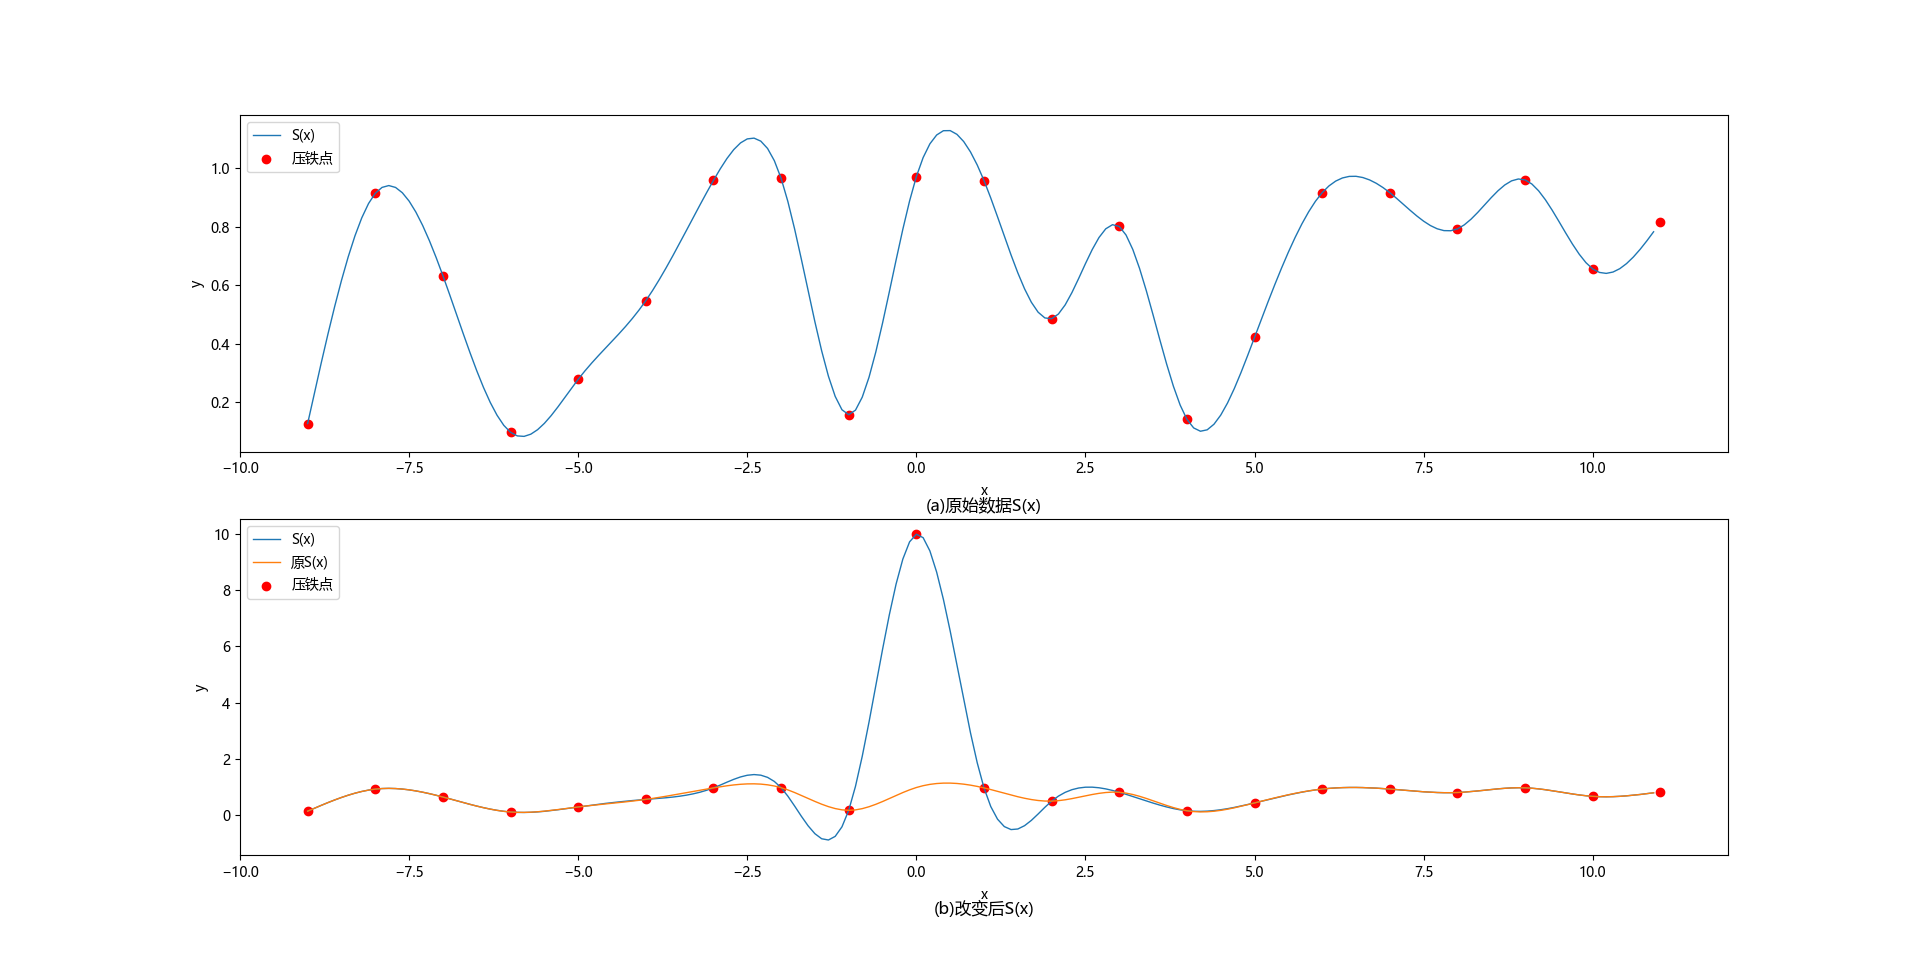
\includegraphics[scale=0.4]{S}
	\captionsetup{font={small},labelfont=bf}
	\caption{\heiti\zihao{-5}压铁结果曲线}
	
\end{figure}


根据计算结果和绘制出的曲线图可以得到,在第十个压铁的邻近两个区间中的函数以及趋势有明显的变化,而到了相隔一个区间的位置,两次S的差异已经明显缩小,趋势已经基本一致。到了相隔3个区间以上时,可以发现两次的拟合函数之间基本已经不存在差异。由此可见三次样条插值局部较为独立稳定。
\end{document}